\documentclass{article}
\usepackage{fancyhdr,booktabs}
\usepackage{amsmath}
\usepackage{float}
\usepackage{graphicx}
\usepackage{indentfirst}
\usepackage{geometry}
\usepackage{citesort}

\begin{document}

\section{Introduction}
\section{Numerical Method}
In this section we describes how we generate EMRI waveforms in non-Kerr metric and process EMRI signal. In \ref{p_krz}, a continuously parametrized metric proposed by \cite{KRZ} is introduced, in \ref{p_kludge}, the method to generate EMRI waveforms proposed by \cite{kludge} is described and \ref{p_mf} summarizes the signal processing pipeline.
\subsection{Konoplya-Rezzolla-Zhidenko parametrization}
\label{p_krz}
In order to test Kerr hypothesis or General Relativity, one need an alternative theory or a non-Kerr metric. Here we use the metric parametrization proposed by Konoplya, Rezzolla and Zhidenko (see \cite{KRZ}) and still calculate the gravitational wave within General Relativity. 

The line element around an axisymmetric black hole in KRZ parametrization is \cite{KRZ}:
\begin{equation}
	ds^2=-\frac{N^2(r,\theta)-W^2(r,\theta)\sin^2\theta}{K^2(r,\theta)} dt^2-2W(r,\theta)r\sin^2\theta dtd\phi + K^2(r,\theta) r^2\sin^2\theta d\phi^2 \\ +\Sigma(r,\theta)(\frac{B^2(r,\theta)}{N^2(r,\theta)} dr^2+r^2d\theta^2)
\end{equation}
Where the functions $K(r,\theta),\, N(r,\theta),\, W(r,\theta),\, B(r,\theta),\, \Sigma(r,\theta) $ can be expanded by power series of $\cos\theta$. Here we use the same deformation parameter as \cite{cosimoKRZ}, namely $\delta_i, \, i=1,2,3,4,5,6$ related to the metric functions by
\begin{equation}
\begin{aligned}
N^2=(1-r_0/r)[ 1-\epsilon_0r_0/r +(k_{00}-\epsilon_0)r_0^2/r^2 +\delta_1 r_0^3/r^3 ] \\
+ \{ a_{20} r_0^3/r^3 +a_{21} r_0^4/r^4 + k_{21}r_0^3/r^3[ 1+\frac{k_{22}(1-r_0/r) }{1+k_{23}(1-r_0/r)} ]^{-1}   \} \cos^2\theta   \\
B=1+\delta_4r_0^2 /r^2 +\delta_5r_0^2 \cos^2\theta /r^2\\
\Sigma = 1+a^2\cos^2\theta /r^2\\
W=[w_{00}r_0^2 /r^2 +\delta_2 r_0^3/r^3 +\delta_3 r_0^3/r^3 \cos^2\theta ]/\Sigma\\
K^2= 1+aW/r+\{k_{00}r_0^2/r^2 +k_{21}r_0^3/r^3 [ 1+\frac{k_{22}(1-r_0/r) }{1+k_{23}(1-r_0/r)} ]^{-1} \cos^2\theta \}/\Sigma\\
r_0=1+\sqrt{1-a^2},\,\,\, a_{20}=2a^2/r_0^3,\,\,\, a_{21}=-a^4/r_0^4 +\delta_6 ,\,\,\, \epsilon_0=(2-r_0)/r_0,\,\,\, k_{00}=a^2/r_0^2,\\
 k_{21}=a^4/r_0^4 -2a^2/r_0^3-\delta_6,\,\,\, w_{00}=2a/r_0^2,\,\,\, k_{22}=-a^2/r_0^2 +\delta_7,\,\,\,  k_{23} = a^2/r_0^2 +\delta_8
\end{aligned}
\end{equation}

KRZ parametrization preserves stationarity and axisymmetry. When each $\delta_i$ is set to 0, the metric recovers Kerr metric. In this paper we mainly consider influence of $\delta_1, \, \delta_2$.

\subsection{"Kludge" Waveform}
\label{p_kludge}
We use the method established in \cite{kludge}, i.e. Kludge waveform, to calculate EMRI waveforms. The procedure is: regarding the stellar mass object as a point particle, first calculate the trajectory of the particle in a given metric by integrating geodesic equations; then use quadruple formula to get the gravitational wave from geodesics.

In our instance, to calculate the geodesics, we use:
\begin{equation}
	\dot{u^\mu}=-\Gamma^\mu_{\rho\sigma}u^\rho u^\sigma
\end{equation}
\begin{equation}
	\dot{x^\mu}=u^\mu 
\end{equation}
where $x^\mu$ is the Boyer-Lindquist coordinate of the particle, $u^\mu$ is the 4-velocity and $\Gamma^\mu_{\rho\sigma}$ is Christoffel connection. We didn't use conservation of particle mass, energy and angular momentum to reduce equation but to monitor numerical error. Namely at each step of integration, we check the conservation quantities defined by:
\begin{equation}
	\eta = g_{\mu\nu} u^\mu u^\nu
\end{equation}
\begin{equation}
	E = -u_t = - g_{tt} u^t -g_{t\phi} u^\phi
\end{equation}
\begin{equation}
	Lz = u_\phi = g_{t\phi } u^t + g_{\phi\phi} u^\phi
\end{equation}
 and in Kerr cases, we also check Carter constant
 \begin{equation}
 	Q = (g_{\theta\theta} u^\theta)^2 + \cos ^2 \theta (a^2 (\eta^2-E^2) + (\frac{Lz}{\sin \theta})^2 )
 \end{equation}
During the calculation, we keep the relative drift of conserved quantities less than $10^{-7}$.

For stable bounded geodesics, three parameters, i.e. eccentricity $e$, semi-latus $p$ and inclination angle $\iota$, can be used to characterize the orbit. They are defined as:
\begin{equation}
\begin{aligned}
e=\frac{r_a-r_p}{r_a+r_p},\,\,\, p=\frac{2r_a r_p}{r_a+r_p},\,\,\, \iota=\frac \pi 2 -\theta_{min}
\end{aligned}
\end{equation} 
where $r_a$ is apastron, $r_p$ is periastron and $\theta_{min}$ is the minimum of $\theta$ coordinate. In Kerr spacetime, we can determine the three orbit parameters $e,p,\iota$ from three conserved quantities $E,L_z,Q$ and vice versa. In KRZ non-Kerr spacetime, for equatorial orbits, we can still determine $e,p$ by $E,L_z$.

Transform $(r,\,\theta,\,\phi)$ into $(x,\,y,\,z)$ with the definition of spherical coordinate (rather than the Boyer-Lindquist coordinate), namely $x=r\sin\theta \cos \phi,\, y=r\sin\theta\sin\phi,\, z=r\cos\theta$. Then use quadruple formula, transform the waveform into transverse-traceless gauge (see formula (17) and (23) in \cite{kludge}), and we get the plus and cross component of the waveform. With the resulted "plus" and "cross" components, we define our waveform as $h = h_+ + i h_\times$
\subsection{Signal Analysis}
\label{p_mf}
Matched filtering is the standard technique to be used in LISA analysis. Here we mainly adopt the filling factor as  a measure of similarity between two waveforms within LISA band. 

The inner product between two signals, a(t) and b(t), is defined by their cross correlation: \cite{product}
\begin{equation}
	(a|b)=4\Re\int \frac{\tilde{a}^*(f) \tilde{b}(f)}{S_n(f)}df =2\int \frac{\tilde{a}^*(f) \tilde{b}(f) +\tilde{a}(f) \tilde{b}^*(f) }{S_n(f)}df
\end{equation}
where $S_n(f)$ is the power spectral density of LISA noise. In our calculation, the analytic fit to the noise spectrum same as \cite{kludge} is used.

The overlap (filling factor) between two EMRIs is defined as:
\begin{equation}
	FF(a,b)=\frac{(a|b)}{\sqrt{(a|a)(b|b)}}
\end{equation}
If the overlap between two waveforms is above 0.97, we regard them as indistinguishable by LISA.

\section{Confusion Problem}
When we try to identify EMRI signals, the confusion problem, as described in \cite{sameOmg}, could prevent us from discern non-Kerr signal and Kerr signal. Namely an overlap over 0.97 might happen between non-Kerr signals and Kerr ones with certain parameters. In \ref{p_2d} and \ref{p_3d} we show the confusion problem when matching EMRIs from equatorial and inclined orbit 
\subsection{Equatorial orbit}
\label{p_2d}
Given a waveform under spacetime with non-zero deformation parameter, in order to see if there is "confusion problem", we need to decide which waveform under Kerr spacetime is most similar to it and look at their overlap. Here we search for existence confusion problem with similar method as \cite{majorPRD}, i.e. looking at waveforms with same orbital frequency. The orbital frequencies in Kerr spacetime are given in \cite{tauOmg}. In equatorial orbits, there are two frequencies $\omega_\phi$ and $\omega_r$ related to motion of $\phi$ and $r$ coordinates.

\begin{figure}[!ht]
	\centering
	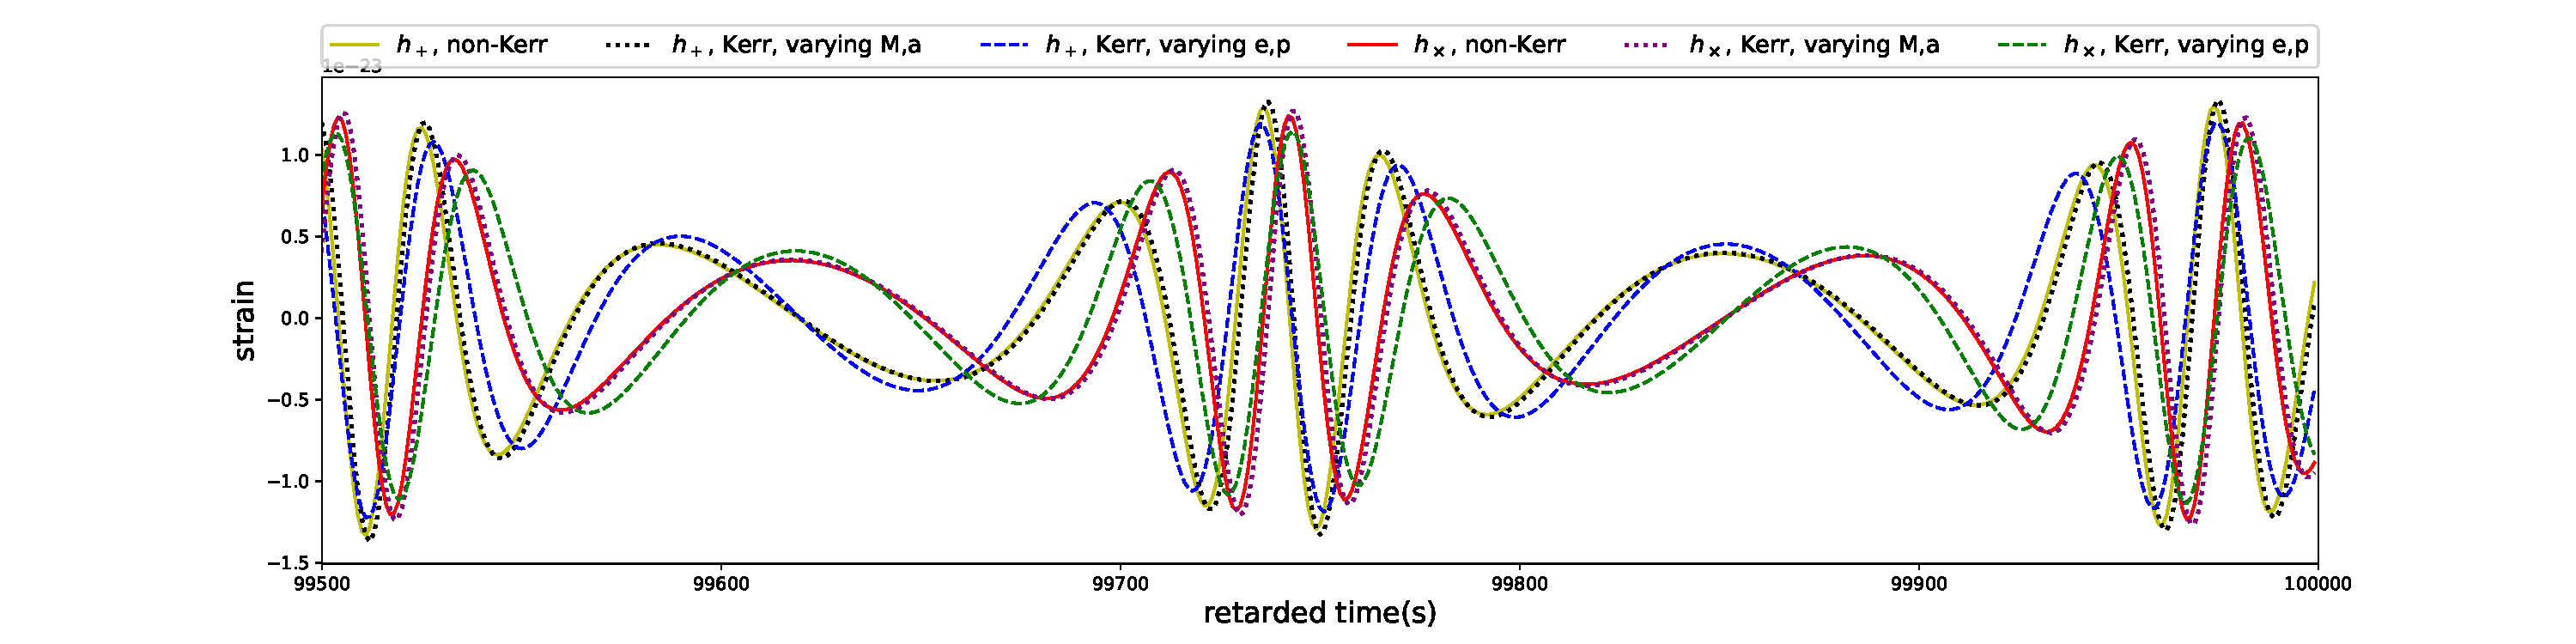
\includegraphics[width=16cm]{eg.pdf}
	
	\caption{"Plus" and "cross" component of EMRIs under non-Kerr spacetime and Kerr spacetime varying $(M,a)$ or $(e,p)$ to equate orbital frequency. The non-Kerr waveform is $(\delta_1,a,M,e,p)=(0,2,0.5,2\times10^5, 0.5,6.0)$. The yellow and red solid lines are "plus" and "cross" component of the non-Kerr waveform. The black and violet dotted lines are "plus" and "cross" component of Kerr waveform with same orbital frequencies as non-Kerr orbit by varying $(M,a)$. The blue and green dashed lines are "plus" and "cross" component of Kerr waveform with same orbital frequencies as non-Kerr orbit by varying $(e,p)$ }
	\label{kkwave}
\end{figure}	

If we restrict ourselves to equatorial motion, set the initial $t$ and $\phi$ to 0 in view of stationarity and axisymmetry and set initial $r=r_{max}$, then the orbit is uniquely determined by orbital eccentricity $e$, semilatus rectum $p$, deformation parameters $\delta_i$, BH mass $M$ and BH spin $a$. As described in \cite{majorPRD}, we can achieve same orbital frequency as non-Kerr signal by varying orbital parameters $e, \,p$ or BH parameters $M, \, a$. So we need to consider EMRIs determined by $(\delta,\, a,\, M,\, e,\, p)$, $(0,\, a,\, M,\, e_{Kerr},\, p_{Kerr})$ and $(0,\, a_{Kerr},\, M_{Kerr},\, e,\, p)$. Comparison of waveforms of same orbital frequency is show in Fig. \ref{kkwave}. The overlap between waveforms varying BH mass and spin is over 0.99. In fact, the geodesics that generate the two waves are overlapping.  

\begin{figure}[htb]
	\centering
	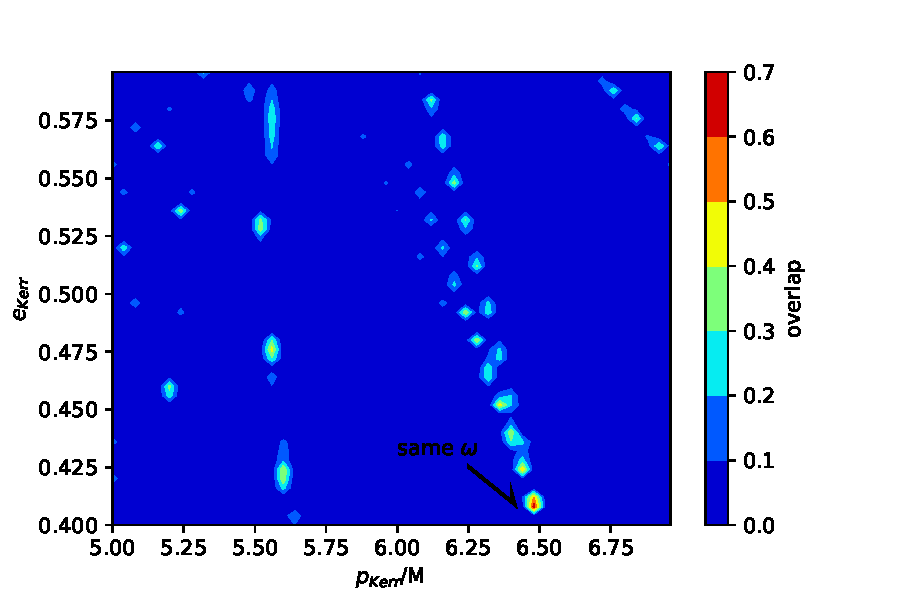
\includegraphics[width=7cm]{OLdist.pdf}
	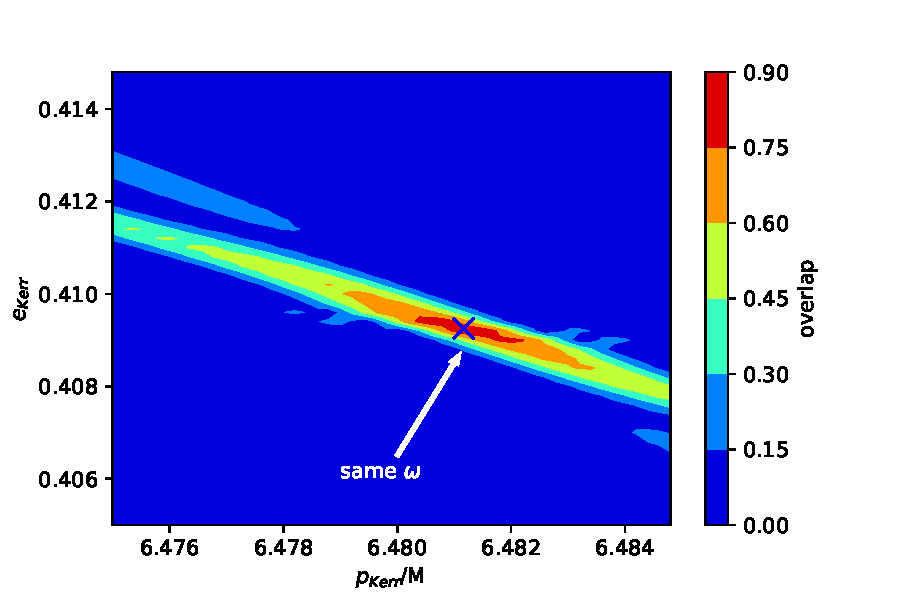
\includegraphics[width=7cm]{OLdist2.pdf}
	
	\caption{Distribution of overlap between waveform of ($\delta_1,\, a,\, M,\, e,\, p$) = (0.2, 0.5, $2 \times 10^5 $, 0.5, 6) and waveforms of ($\delta_1,\, a,\, M,\, e,\, p$) =(0, 0.5, $2 \times 10^5 $, $e_{Kerr}$, $p_{Kerr}$) on ($e_{Kerr}$, $p_{Kerr}$) plane. blue cross mark pointed by the arrow: same $\omega_r$ and $\omega_\phi$ at ($e_{Kerr}$, $p_{Kerr}$) = (0.409248, 6.481170).  The grid size is 50*50.}
	\label{overlapdist}
\end{figure}

According to Ref. \cite{sameOmg}, orbits with same orbital frequency $\omega_r$ and $\omega_\phi$ can generate gravitational waveforms potentially confused with non-Kerr signals. Therefore the overlap between a non-Kerr waveform and several Kerr waveforms should have a local maximum around the parameter leading to same orbital frequency. Here we check this result by looking at overlaps between waveform of ($\delta_1,\, a,\, M,\, e,\, p$) = (0.2, 0.5, $2 \times 10^5 $ , 0.5, 6) and of ($\delta_1,\, a,\, M,\, e,\, p$) = (0, 0.5, $2 \times 10^5 $ , $e_{Kerr}$, $p_{Kerr}$) with varying $e_{Kerr}$ and $p_{Kerr}$. First we look at overlap distribution on a relatively large range of (e, p). Then we search near ($e_{Kerr}$, $p_{Kerr}$) with same orbital frequency, as shown in Fig. \ref{overlapdist}. 

	\begin{figure}[!h]
	\centering
	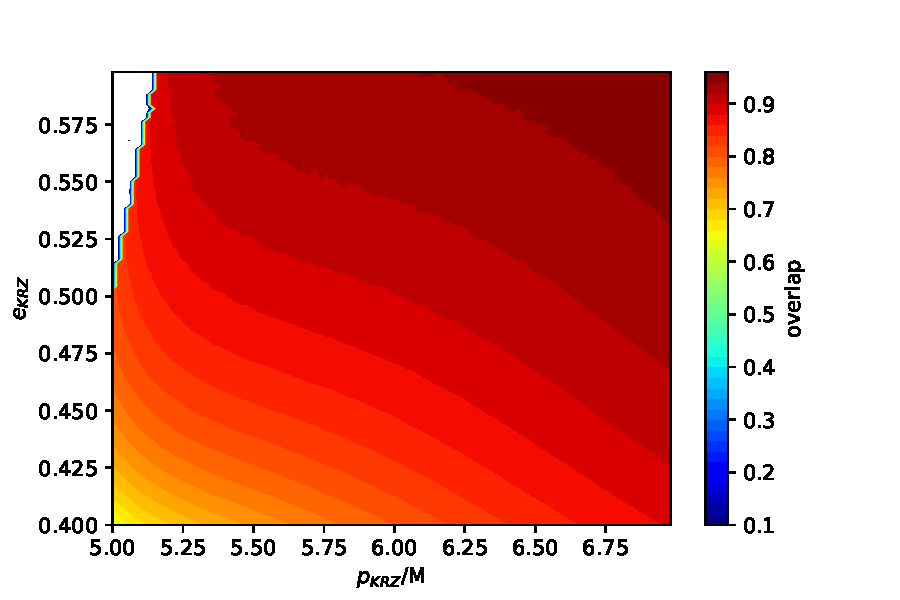
\includegraphics[width=10cm]{ep_best_dist.pdf}
	
	\caption{distribution of overlap between waveform of ($\delta_1,\, a,\, M,\, e,\, p$) = (0.2, 0.5, $2 \times 10^5 $ , $e_{KRZ}$, $p_{KRZ}$) and Kerr waveform with identical $\omega_r$ and $\omega_\phi$ by varying $e_{Kerr},\, p_{Kerr}$. The grid size is 100*100. The blank region is unstable orbits.}
	\label{epdist}
\end{figure}	

	\begin{figure}[!ht]
	\centering
	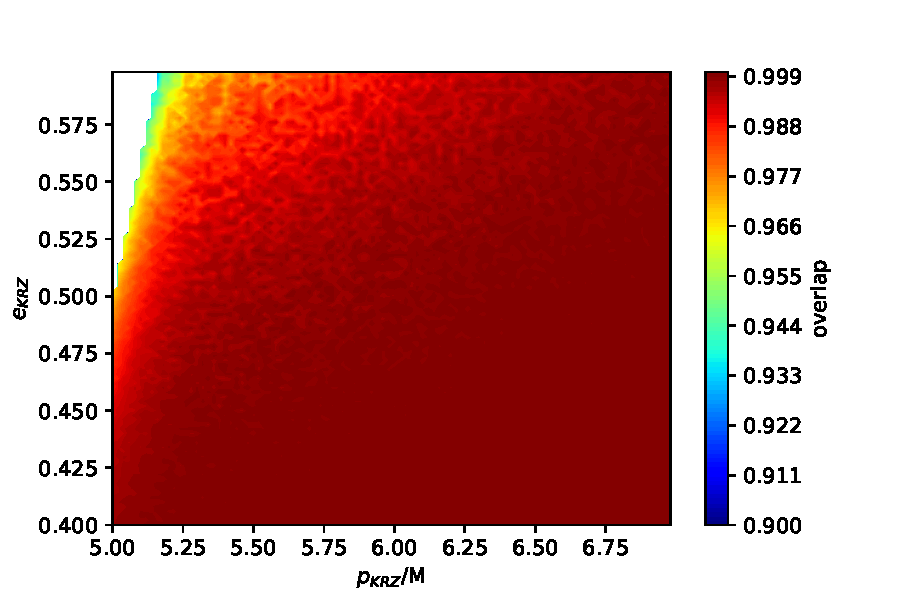
\includegraphics[width=10cm]{FF_am.pdf}
	
	\caption{distribution of overlap between waveform of ($\delta_1,\, a,\, M,\, e,\, p$) = (0.2, 0.5, $2 \times 10^5 $ , $e_{KRZ}$, $p_{KRZ}$) and Kerr waveform with identical $\omega^{(t)}$ by varying $M_{Kerr},\, a_{Kerr}$. The grid size is 100*100. The blank region is unstable orbits.}
	\label{amdist}
\end{figure}	

Since metric deformation is more evident near BH horizon, we look at waveforms generated by trajectories close to innermost bound orbit. We compare waveforms of ($\delta_1,\, a,\, M,\, e,\, p$) = (0.2, 0.5, $2 \times 10^5 $ , $e$, $p$) and Kerr orbits varying $(e,p)$ or $(M,a)$ in a 50*50 grid of $(e,p)$. Contour plots of waveform overlap when varying $(e,p)$ and $(M,a)$ are shown in Fig. \ref{epdist} and \ref{amdist}. The confusion problem exists when varying $(M,a)$ for most region we considered. 

\begin{figure}[!ht]
	\centering
	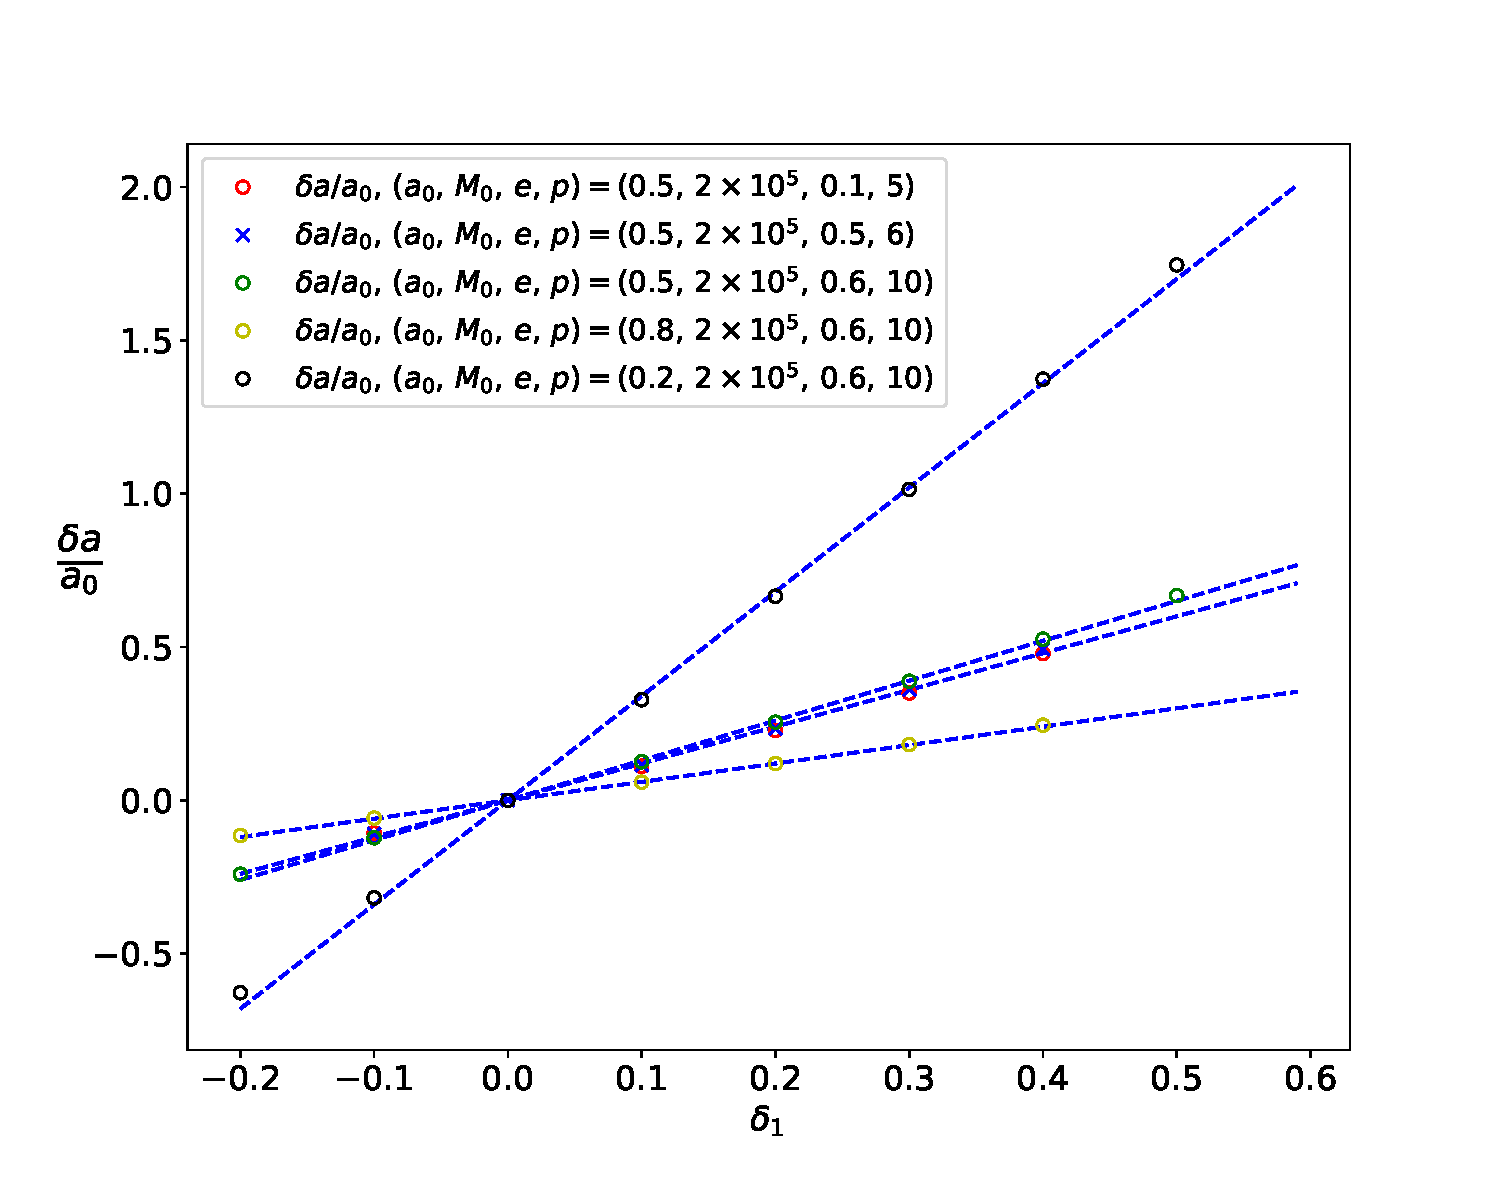
\includegraphics[width=7cm]{d1_spin_linear.pdf}
	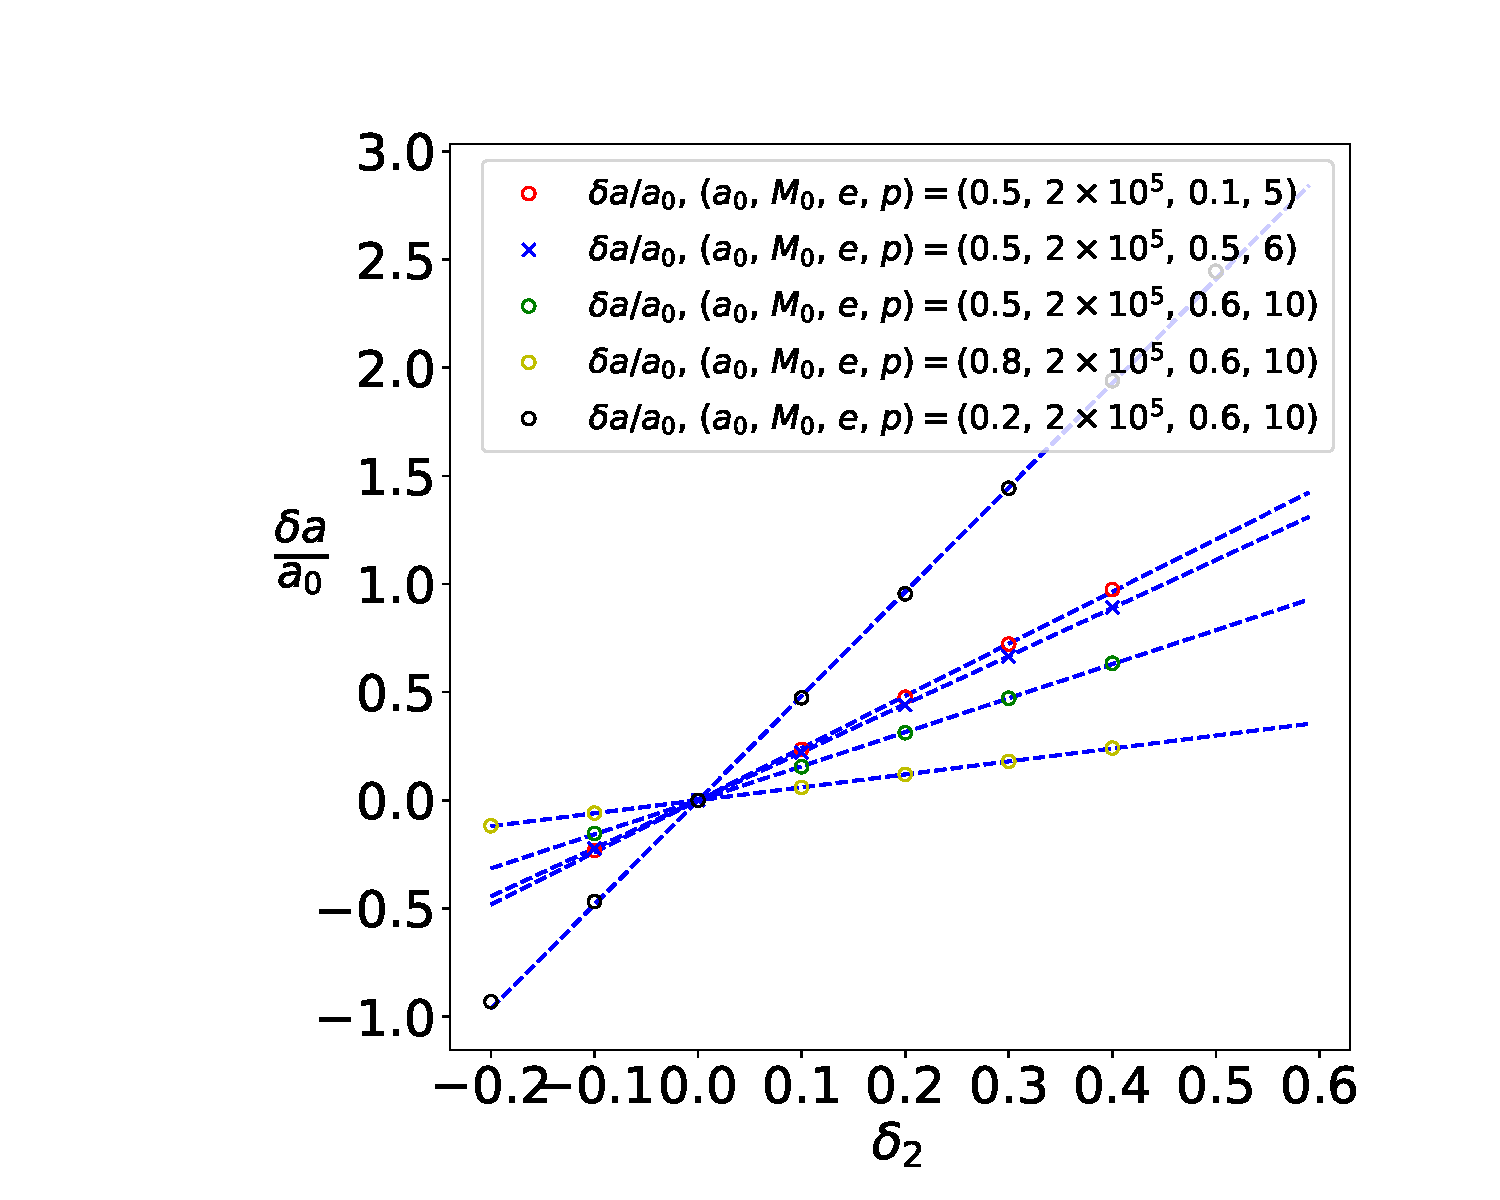
\includegraphics[width=7cm]{d2_spin_linear.pdf}
	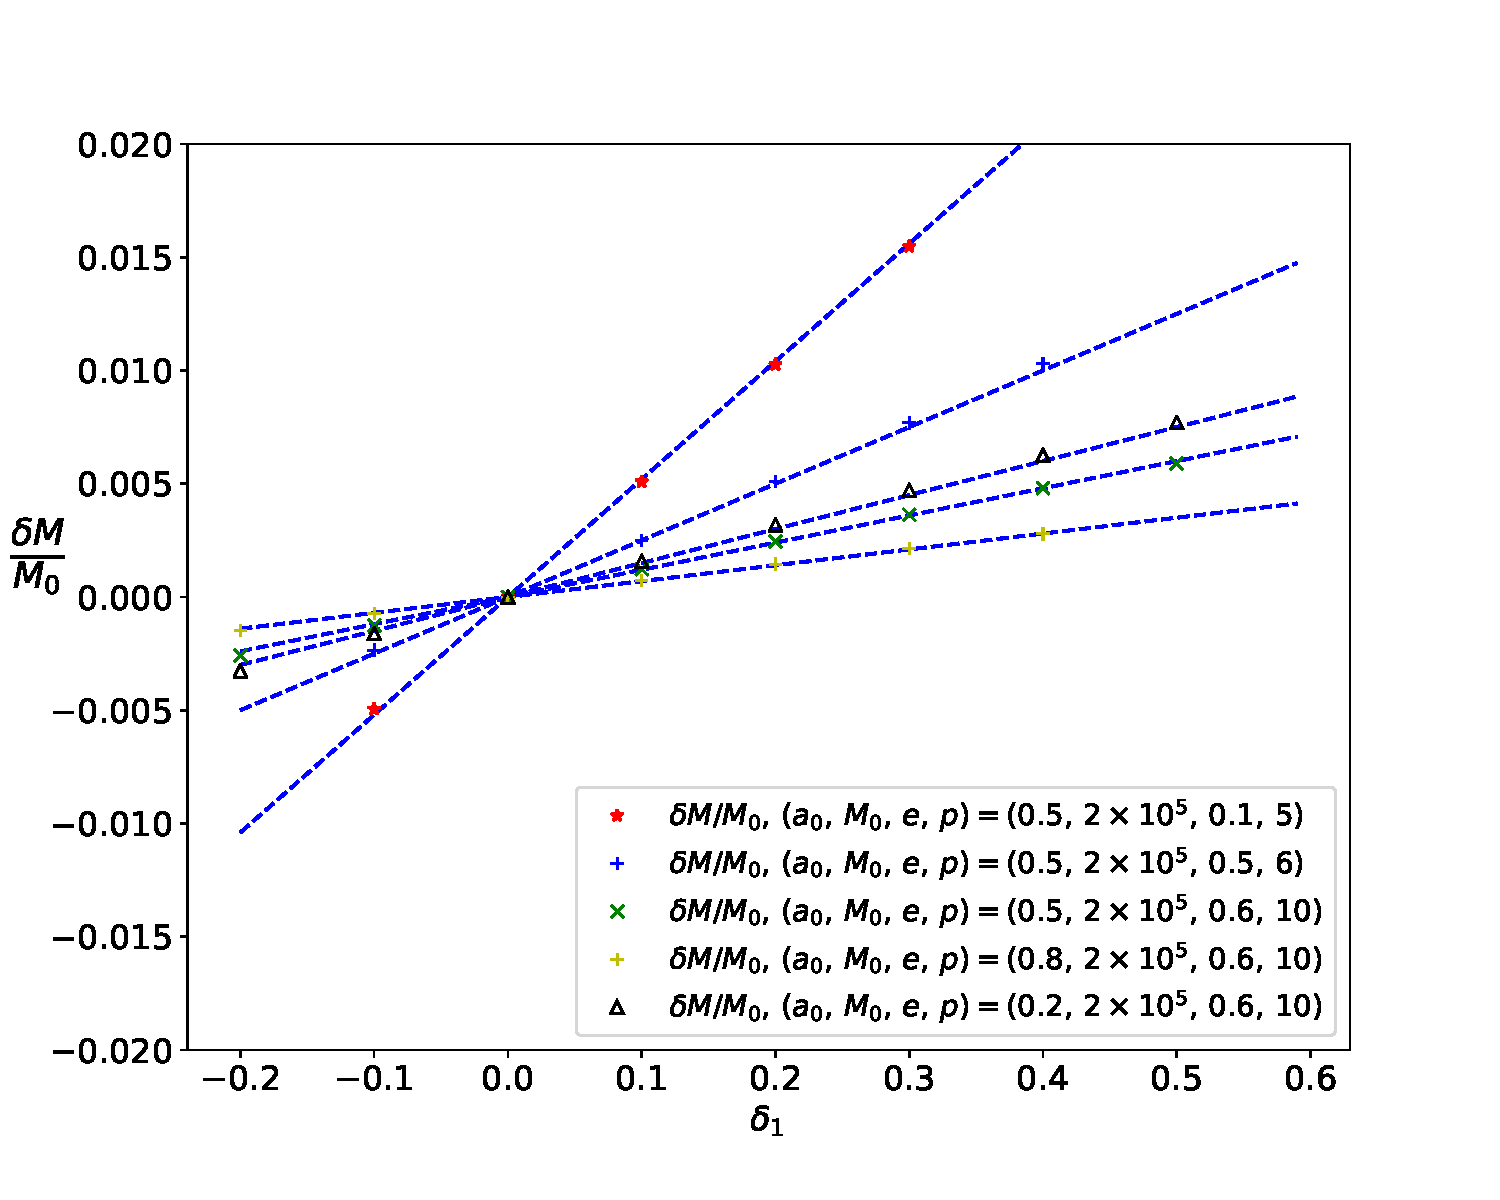
\includegraphics[width=7cm]{d1_M.pdf}
	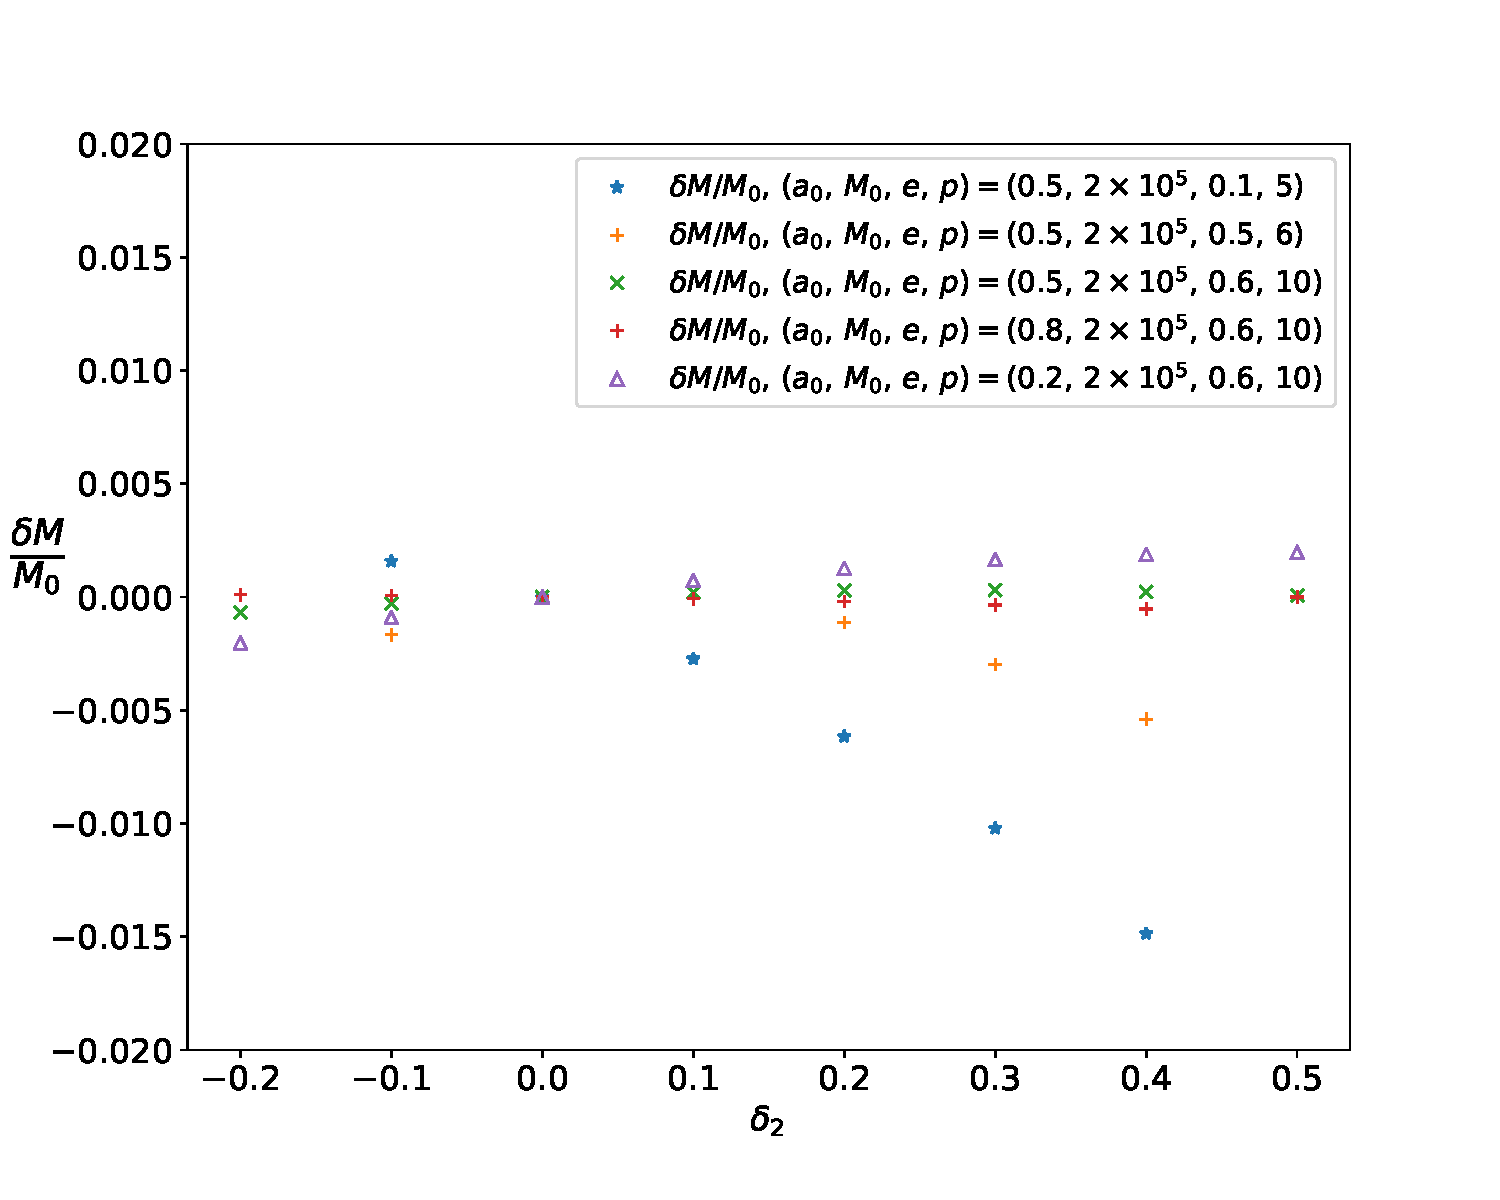
\includegraphics[width=7cm]{d2_M.pdf}
	\caption{relation between relative varied spin/Mass when equating orbital frequency, i.e. orbit of $(\delta_i, a_0, M_0,e,p)$ and $(0,a_0+\delta a, M_0+\delta M,e,p)$ have same orbital frequencies and here shows $\frac{\delta a}{a_0}$-$\delta_i$ or $\frac{\delta M}{M_0}$-$\delta_i$ relations. top left panel: relations of $\frac{\delta a}{a_0}$ or $\frac{\delta M}{M_0}$ to $\delta_1$, top right panel: relations of $\frac{\delta a}{a_0}$ or $\frac{\delta M}{M_0}$ to $\delta_2$.}
	\label{da_linear}
\end{figure}

\begin{figure}[!ht]
	\centering
	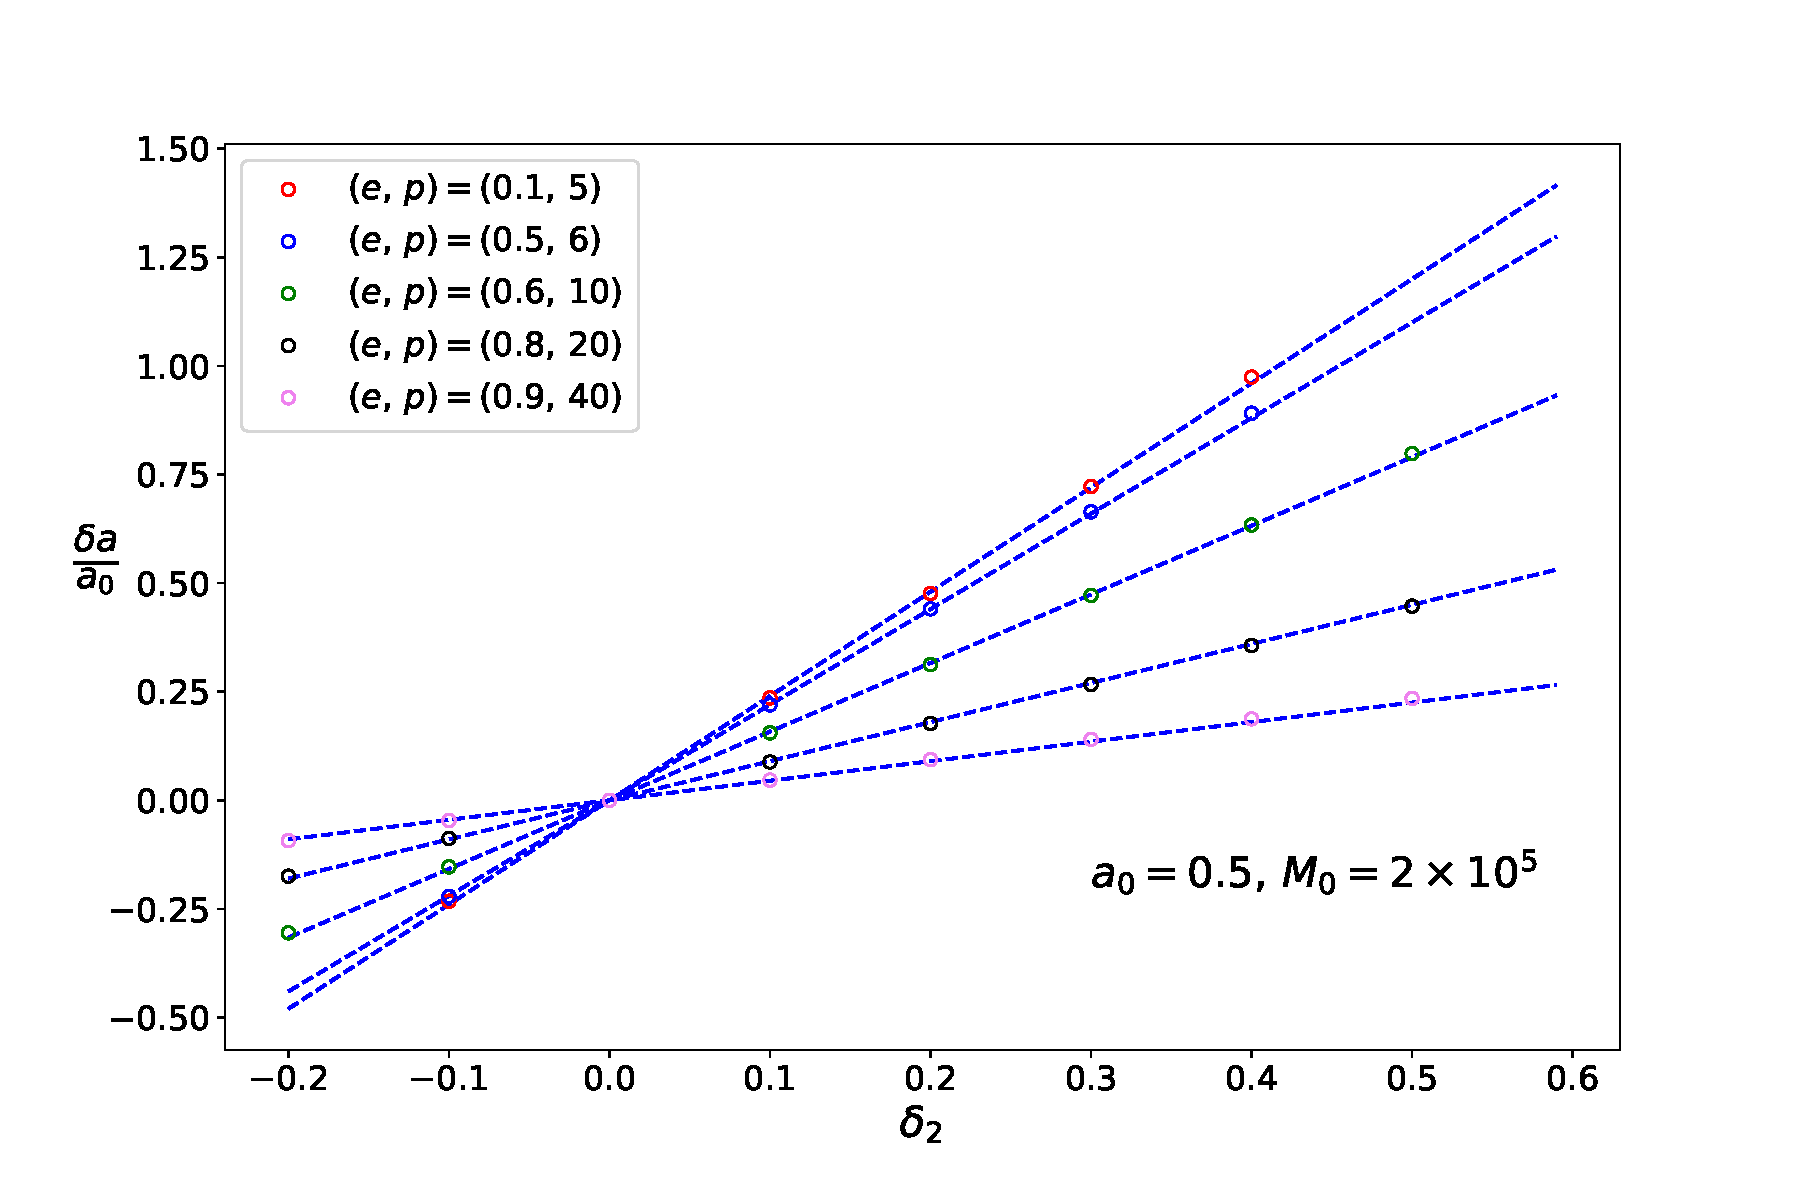
\includegraphics[width=8cm]{d2_deltaspin_ep.pdf}
	
	\caption{Same as Fig. \ref{da_linear}, but only for $\delta a/a_0$-$\delta_2$ relations for different orbits.}
	\label{ep_slope}
\end{figure}

Furthermore, the confusion problem exists for a large range of deformation parameter. When changing the deformation parameter, we found a almost linear relation between $\delta_i$ and varied BH spin/mass, $a_{Kerr}$ and $M_{Kerr}$, as shown in Fig. \ref{da_linear}. Fig. \ref{ep_slope} shows that slope of this "linear" relation varies greatly for different $(e,\,p)$, so the relation is not a property intrinsic to the metric but dependent on the orbit. The linearity is not a result of small deformation. In fact, as shown in the two figures, the spin varies up to one or two times the spin in KRZ metric. 

\begin{figure}[!ht]
	\centering
	\includegraphics[width=7cm]{2D_bound.pdf}
	\includegraphics[width=7cm]{2D_bound_d2.pdf}
	
	\caption{Upper and lower limit of $\delta_i$, whose waveform can be confused with Kerr waveform, on $delta_i$-$a_{KRZ}$ parameter plane, set by equatorial orbit requiring $a_{Kerr}<1$ and stable orbit. Other parameters are set to: eccentricity $e=0.5$, semi-latus $p=6.0$ and Balck hole mass $M=2\times10^5$ solar mass. Waveforms in red parameter region, when trying to equate orbital frequencies by varying $(M,a)$, results in $a_{Kerr}$ larger than 1. Waveforms in blue region can be confused with Kerr waveform. Orbits in yellow region do not exist. Left panel: for $\delta_1$ and $\delta_2$ set to 0. Right panel: for $\delta_2$ and $\delta_1$ set to 0. }
	\label{d2limit}
\end{figure}

Therefore, for a given orbit parameter $(e,\, p)$, we can regard the introduction of $\delta_i$ as adding the black hole spin and mass proportionally. This sets an limit for the range of deformation parameters within which we can play the trick of varying $(M_{Kerr},\, a_{Kerr})$. The upper limit is set by requiring $a_{Kerr}<1$ and the lower is limited by $a_{Kerr}>0$ or stable orbit, e.g. for $(e,\, p)=(0.5,\, 6.0)$, when $a_{Kerr}$ is small, the orbit is no longer stable and bounded. Fig. \ref{d2limit} shows the upper and lower bound of deformation parameters with respect to BH spin for orbit with $e=0.5,\, p=6.0$. 

\subsection{Inclined orbit}
\label{p_3d}
Equatorial orbits set some special conditions, i.e. number of orbital frequencies is equal to number of Kerr BH parameters. Therefore, in general we can solve mass and spin by the two frequency requirements set by KRZ orbit, and the resulted geodesics are almost identical. However, astrophysical EMRIs are usually generated by inclined orbits, which have three orbital frequencies. In such cases we usually cannot equate the three frequencies by only varying BH parameters. 

\begin{figure}[!ht]
	\centering
	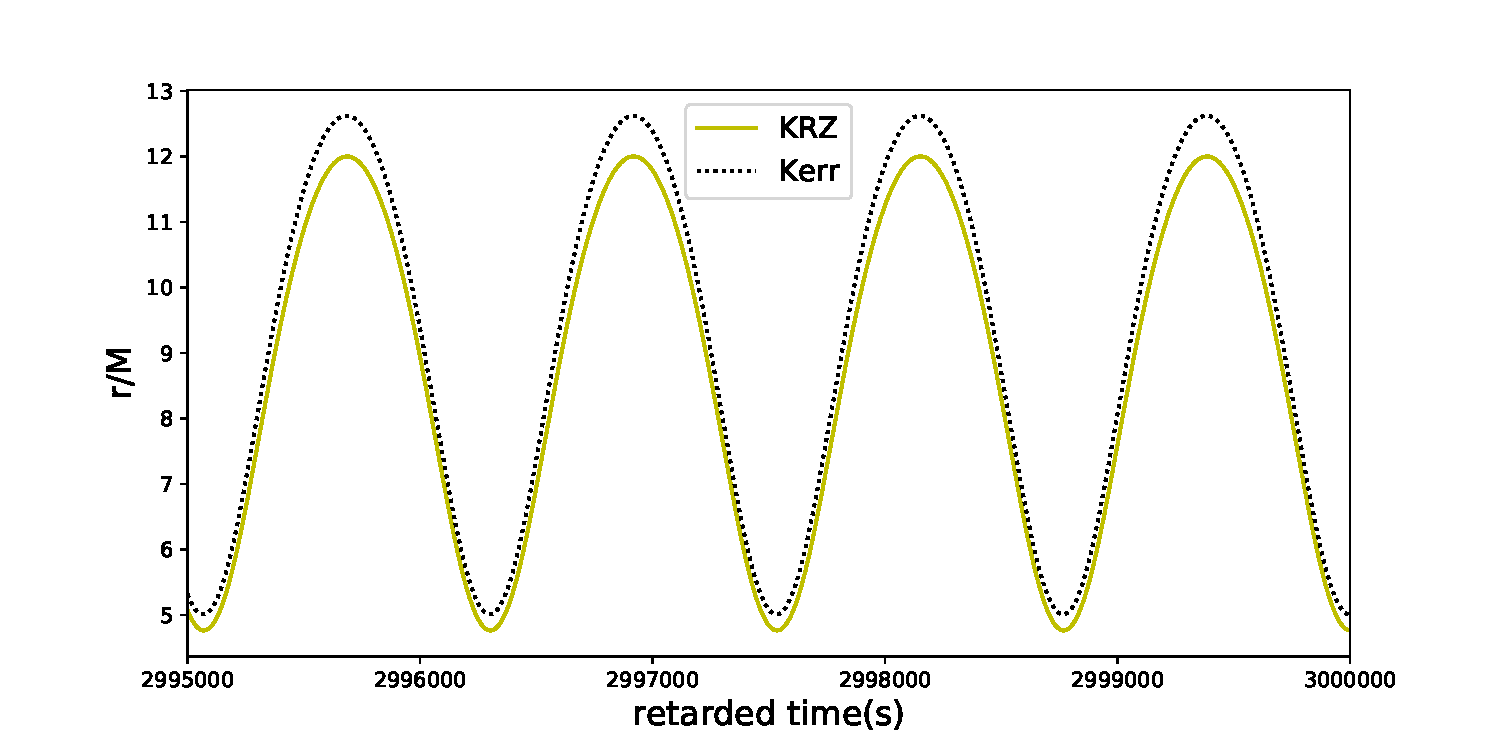
\includegraphics[width=7cm]{r3d.pdf}
	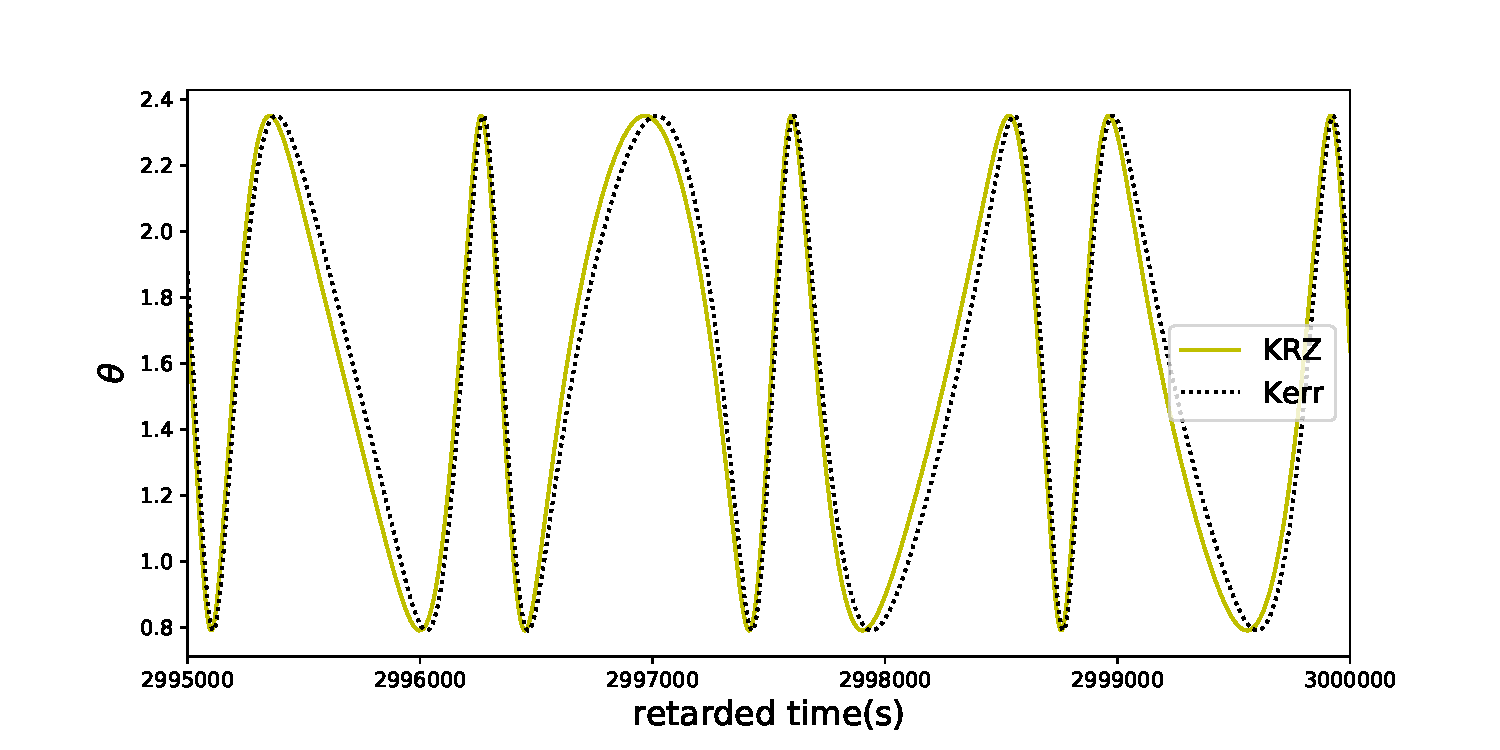
\includegraphics[width=7cm]{th3d.pdf}
	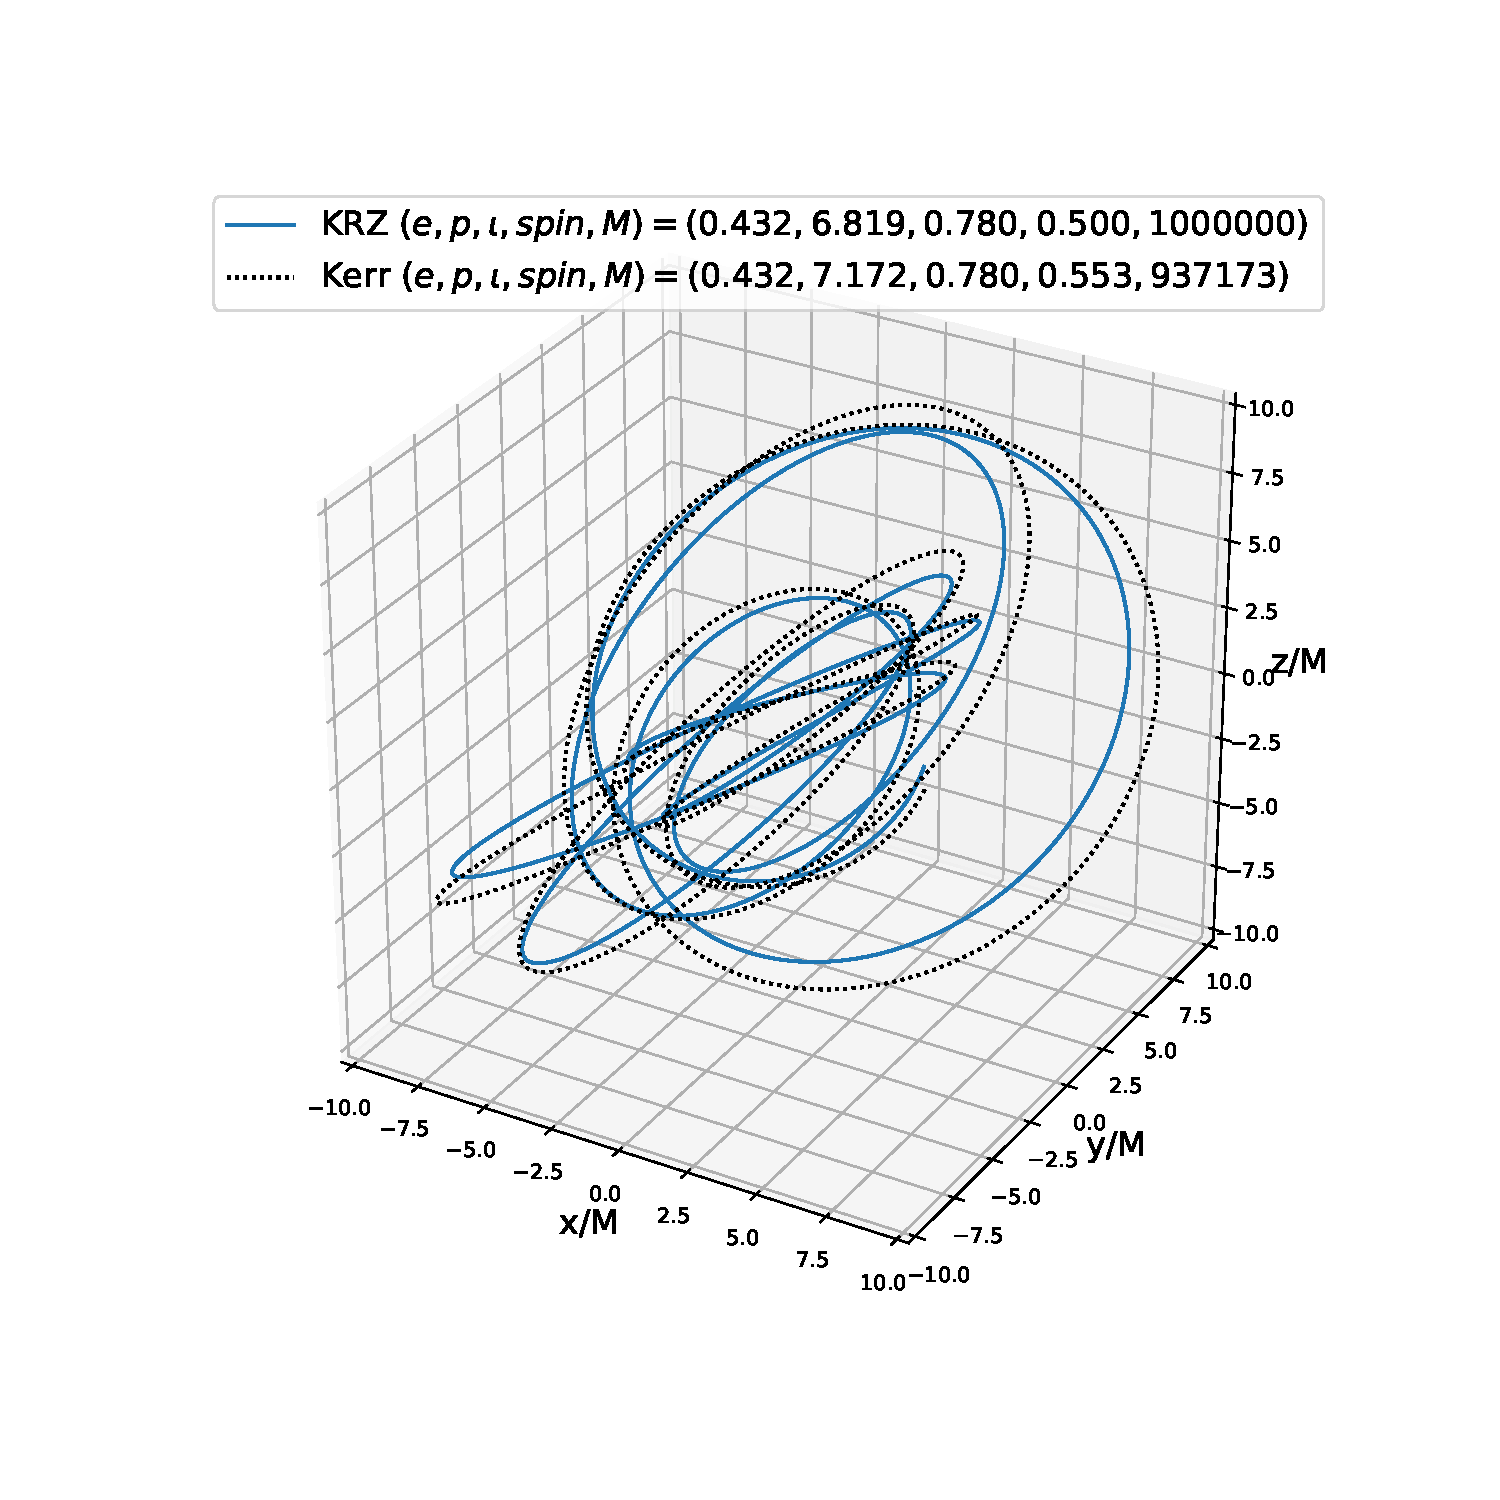
\includegraphics[width=7cm]{trace3d.pdf}
	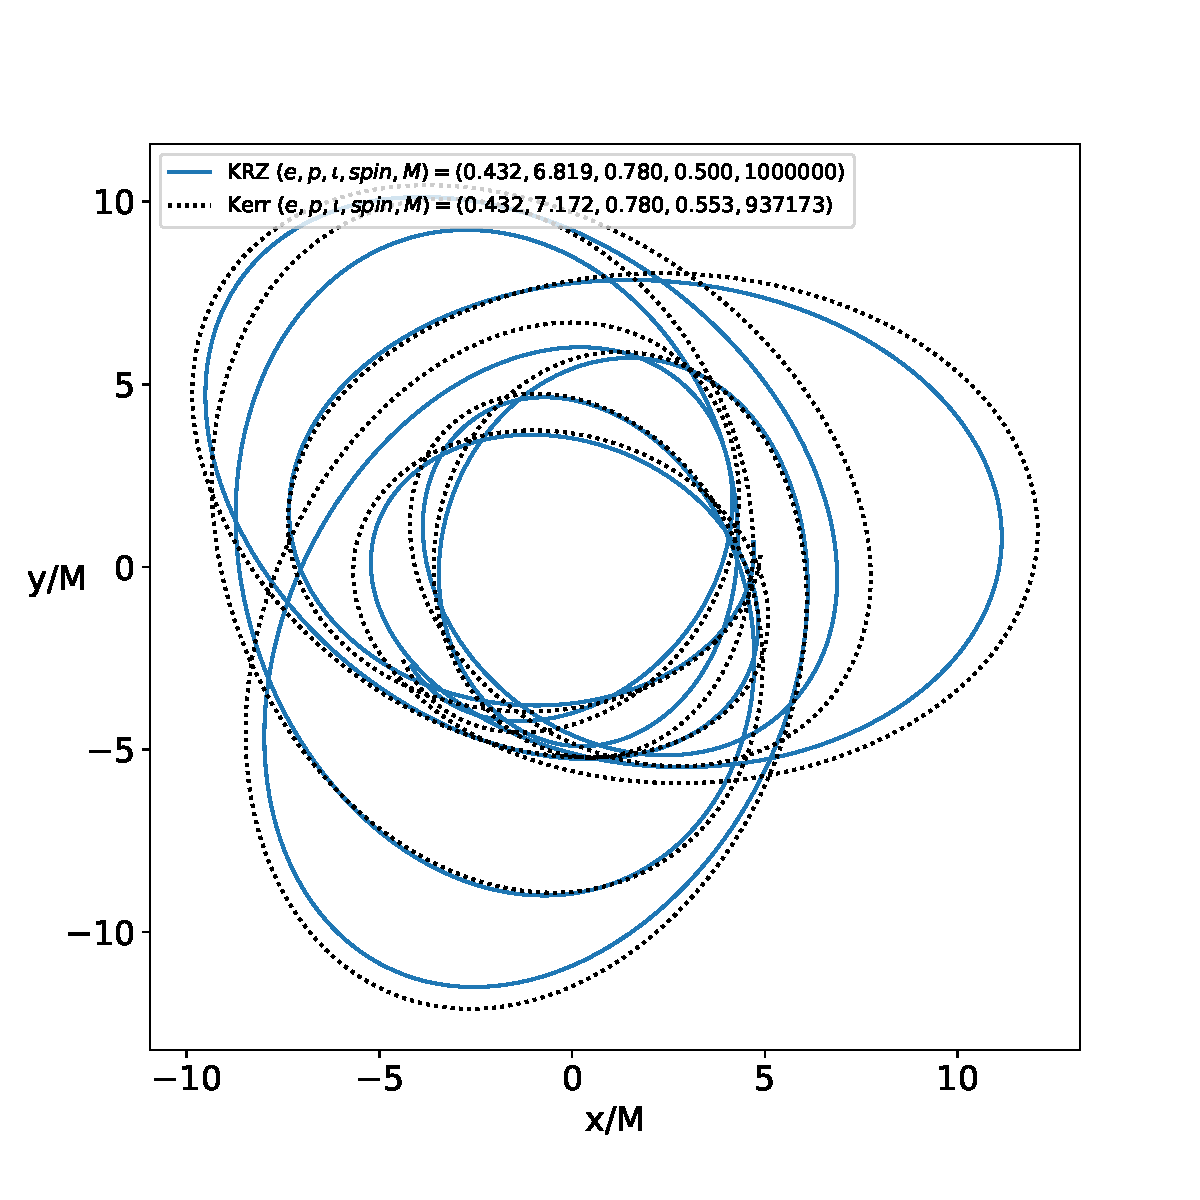
\includegraphics[width=7cm]{tracexy.pdf}
	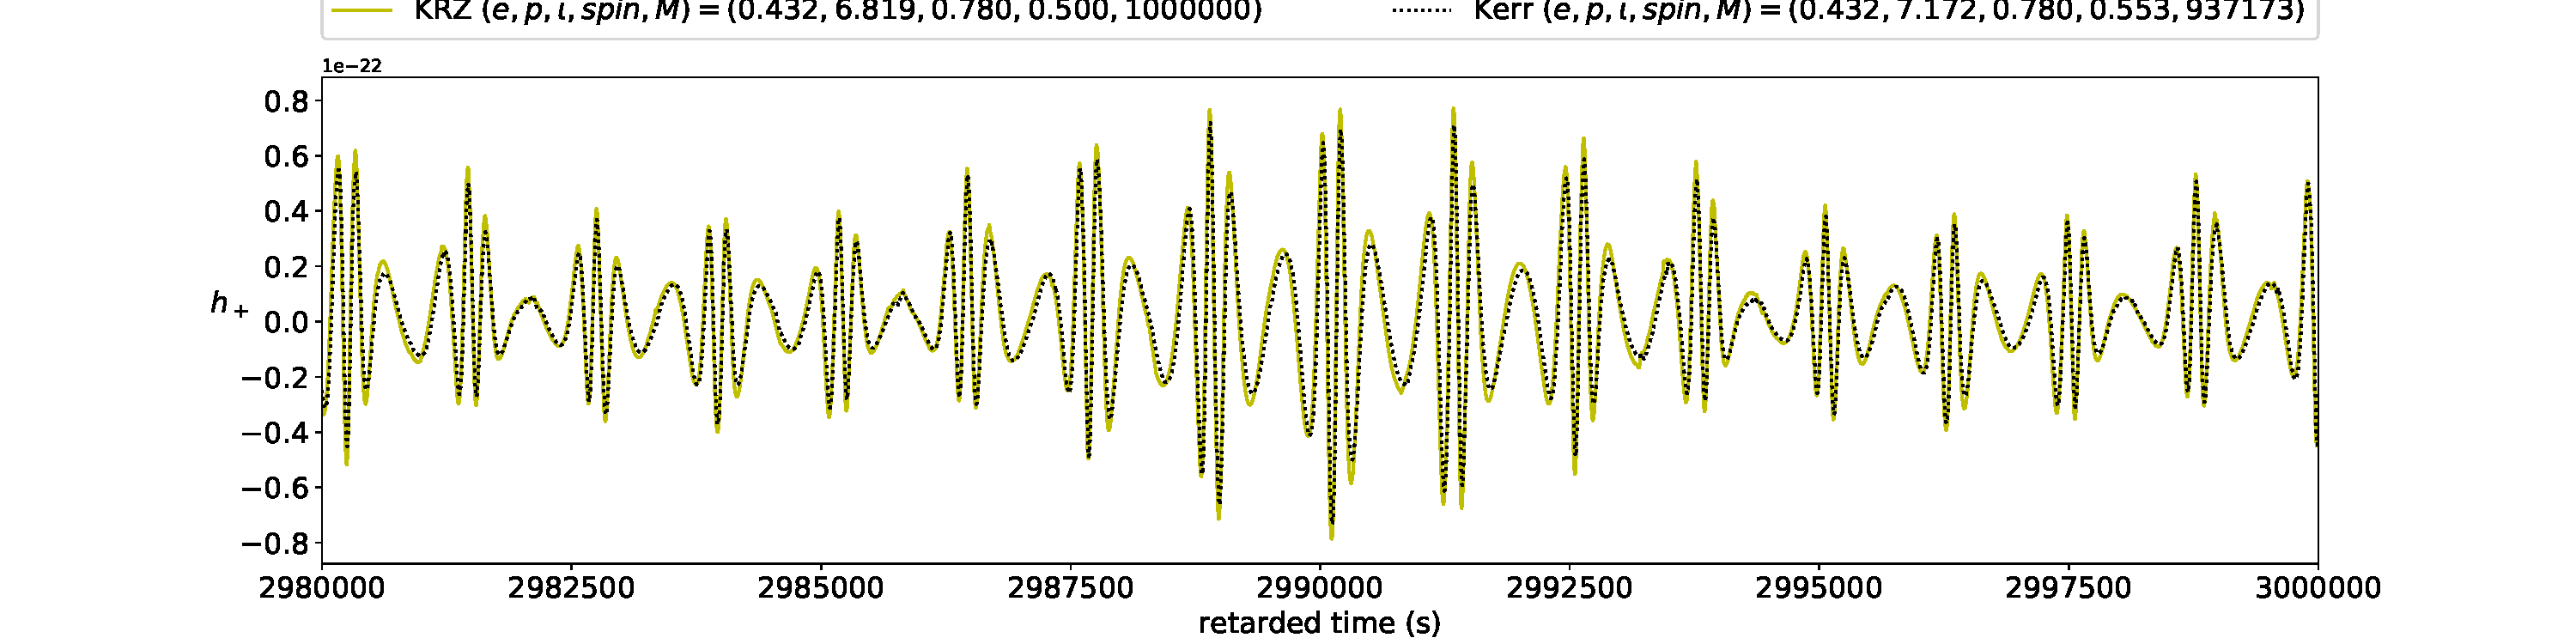
\includegraphics[width=14cm]{wave_d102.pdf}
	
	\caption{Orbits and GW waveforms of a KRZ orbit and a Kerr one with same orbital frequencies. Top left panel: time series of motion in r direction in last 5000s. Top right panel: time series of motion in $\theta$ direction in last 5000s. Middle left panel: trajectories in last 5000s. Middle right panel: projection on xy-plane of the trajectories in last 5000s. Bottom panel: "plus" component of EMRI waveform in last 20000s. The orbit parameters and BH spin/Mass are $(e,p,\iota,spin,M)=(0.432,\, 6.819,\, 0.780,\, 0.5,\, 10^6)$. The deformation parameter of the KRZ orbit is $\delta_1=0.2$.}
	\label{3dtraj}
\end{figure}

However, we found that by varying $(M,\, a,\, p)$ to equate three orbital frequencies, the resulted gravitational waveforms also have an overlap over 0.97, even though the orbits are apparently not identical. Upper and middle panel of Fig. \ref{3dtraj} show the time series of motion in $r,\, \theta $ direction and trajectories in the last 5000s, the total time is $3\times 10^6$s. Motion at $\theta$ direction is almost overlapping with a few distortions. Motion at $r$ direction has the same frequency but different amplitude, basically resulted from varying the semi-latus $p$. However, the gravitational wave signal are almost identical as shown in the bottom panel. 

\begin{figure}[!ht]
	\centering
	\includegraphics[width=8cm]{3D_bound.pdf}
	
	\caption{Same as Fig. \ref{d2limit}, but for inclined orbit and waveform at each point is determined by setting initial $E,Lz$ same as corresponding Kerr orbit, see text for details.}
	\label{3dlimit}
\end{figure}

Similar to equatorial cases, requirements of $a_{Kerr}<1$ and stable orbits set bound to the deformation parameters. However, since there's no carter-like constant in KRZ metric, we cannot control orbit parameters $(e,\, p,\, \iota)$. Therefore, we try just to control the initial condition so that the orbit parameter are at least near the desired value, e.g. $(e,\, p,\, \iota) = (0.2,\, 8,\, \pi/4 )$. Technically, given $\delta_i$, $a_{KRZ}$ and reference orbit parameter, we calculate the energy $E_{Kerr}$ and angular momentum $L_{z -Kerr}$ in Kerr spacetime with spin equal to $a_{KRZ}$, then set the initial coordinate as $\theta=\pi/2$, $\phi=0$, t=0 and r at $\frac{p}{1-e}$, set $E,\, L_z$ equal to the Kerr value, which determines velocity in $t$ and $\phi$ direction, set $u^r=0$ and $u^\theta$ is determined by modulus of 4-velocity. The upper and lower bound of deformation parameters determined in this way is shown in Fig. \ref{3dlimit}. $M_{KRZ}$ is $10^6$ solar mass and total time is $2\times 10^6$s.





\bibliography{citation}
\bibliographystyle{plain}
\end{document}